\documentclass{ctexart}
\usepackage{array}
\usepackage{tikz}
\begin{document}
    \uline{汉字下划线.}

    \begin{quote}
        \setlength\extrarowheight{2mm}
        \begin{tabular}{ll}
            班级 & 一年级二班 \\
            \cline{2-2}
            姓名 & 张三 \\
            \cline{2-2}
        \end{tabular}
    \end{quote}

    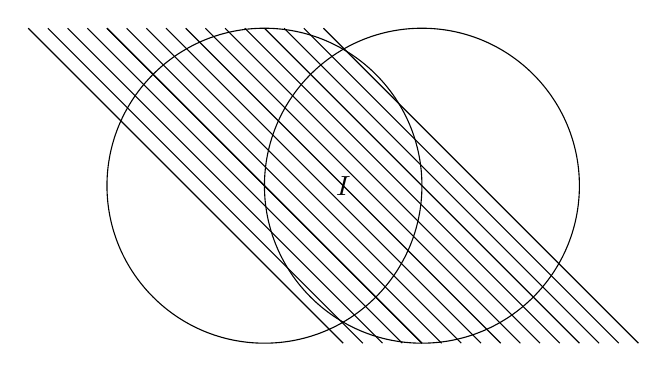
\begin{tikzpicture}
        \draw (0,0) circle (2cm);
        \draw (2,0) circle (2cm);
        % \clip[draw] (0,0) circle (2cm);
        % \clip[draw] (2,0) circle (2cm);
        \foreach \x in {-1,-0.75,-0.5,-0.25,0,0,
            0.25,0.5,0.75,1,1.25,1.5,1.75,2,2.25,2.5,2.75}
        \draw[xshift=\x cm]  (-2,2)--(2,-2);
        \node at (1,0) {$I$};
    \end{tikzpicture}
\end{document}